\documentclass{beamer}

\usetheme{Berlin}
\usecolortheme{Orchid}
\useoutertheme{miniframes}
\setbeamertemplate{navigation symbols}{}

\usepackage[utf8]{inputenc}
\usepackage[T1]{fontenc}
\usepackage{amsmath}
\usepackage{amssymb}
\usepackage{booktabs}
\usepackage{graphicx}
\graphicspath{{../images/}}

\usepackage{xcolor}
\usepackage{listings}
\usepackage{hyperref}
\usepackage{tikz}
\usetikzlibrary{arrows.meta,positioning,shapes.geometric,calc}

\lstset{
  language=Java,
  basicstyle=\ttfamily\small,
  keywordstyle=\color{blue},
  commentstyle=\color{gray},
  stringstyle=\color{teal},
  showstringspaces=false,
  columns=fullflexible,
  breaklines=true
}

% Per-slide source line (references shown on the slide itself).
\newcommand{\slidesources}[1]{%
  \vfill
  {\tiny\color{gray}\raggedright\sloppy\parbox{\linewidth}{Sources: #1}\par}%
}

% Unit-wise source strings for this subject (used by slides/notes).
% Path is relative to the lecture `latex/` folder (the compilation CWD).
% OOPS with Java (CSEG1044) — unit-wise sources
%
% These are short, student-facing reference strings intended to be used with:
%   - \slidesources{...}  (in beamer slides)
%   - \notesources{...}   (in lecture notes)
%
% Style inspiration: other subjects in My-Subjects/ use semicolon-separated sources
% and include an "accessed" date for web documentation.

\newcommand{\OOPSUnitISources}{Schildt, \textit{Java: A Beginner's Guide} (10e), McGraw-Hill (Java fundamentals + OOP basics).; Oracle Java Tutorials: Getting Started + Language Basics + Classes and Objects (accessed \today).; Java SE API docs (e.g., \texttt{String}, \texttt{Scanner}) (accessed \today).}

\newcommand{\OOPSUnitIISources}{Schildt, \textit{Java: The Complete Reference} (12e), McGraw-Hill (classes, inheritance, packages, interfaces).; Bloch, \textit{Effective Java} (3e), Addison-Wesley, 2018 (design choices; interfaces vs abstract classes).; Oracle Java Tutorials: Classes and Objects + Interfaces + Packages (accessed \today).; Java SE API docs (e.g., \texttt{Comparable}, \texttt{Runnable}) (accessed \today).}

\newcommand{\OOPSUnitIIISources}{Schildt, \textit{Java: The Complete Reference} (12e) (nested/inner classes, exceptions, threads, I/O).; Oracle Java Tutorials: Nested Classes + Exceptions + Concurrency + Basic I/O (accessed \today).; Java SE API docs (e.g., \texttt{Thread}, \texttt{AutoCloseable}) (accessed \today).}

\newcommand{\OOPSUnitIVSources}{Schildt, \textit{Java: The Complete Reference} (12e) (generics, lambdas, Swing, JDBC).; Bloch, \textit{Effective Java} (3e) (generics + lambdas).; Oracle Java Tutorials: Generics + Lambda Expressions + Swing + JDBC Basics (accessed \today).; Java SE API docs (e.g., \texttt{java.util.function}, \texttt{javax.swing}, \texttt{java.sql}) (accessed \today).}

\newcommand{\OOPSUnitVSources}{Schildt, \textit{Java: The Complete Reference} (12e) (Collections Framework + wrapper classes).; Oracle Java docs: Collections Framework overview (accessed \today).; Java SE API docs (\texttt{java.util} collections; wrapper classes in \texttt{java.lang}) (accessed \today).}

\newcommand{\OOPSUnitVISources}{Git SCM: \textit{Pro Git} (2e) (version control workflow), accessed \today.; GitHub Docs (repositories, issues, pull requests), accessed \today.; Oracle Java Tutorials: Swing + JDBC (accessed \today).; JUnit 5 User Guide (accessed \today).; Apache Maven Project: Getting Started (accessed \today).; Gradle User Manual: Getting Started (accessed \today).; UML class diagrams: UML 2.x overview/spec (accessed \today).}

\newcommand{\OOPSMiscWhyInterfacesSources}{Schildt, \textit{Java: The Complete Reference} (12e) (interfaces).; Bloch, \textit{Effective Java} (3e) (prefer interfaces where appropriate).; Oracle Java Tutorials: Interfaces (accessed \today).; Java SE API docs (e.g., \texttt{Comparable}, \texttt{Runnable}) (accessed \today).}



\title[OOPS with Java]{Object Oriented Programming (CSEG1044)}
\subtitle{Unit 06 -- Lecture 04: Database Design + JDBC Layer}
\author{Tofik Ali}
\institute{School of Computer Science, UPES Dehradun}
\date{\today}

\begin{document}

\begin{frame}[fragile]
  \titlepage
  \vspace{0.5em}
  \slidesources{\OOPSUnitVISources}
\end{frame}

\begin{frame}{Quick Links}
  \centering
  \hyperlink{sec:overview}{\beamerbutton{Overview}}\hspace{0.6em}
  \hyperlink{sec:concepts}{\beamerbutton{Key Topics}}\hspace{0.6em}
  \hyperlink{sec:demo}{\beamerbutton{Demo}}\hspace{0.6em}
  \hyperlink{sec:summary}{\beamerbutton{Summary}}
  \slidesources{\OOPSUnitVISources}
\end{frame}

\begin{frame}{Agenda}
  \tableofcontents
  \slidesources{\OOPSUnitVISources}
\end{frame}

\section{Overview}
\label{sec:overview}

\begin{frame}{Learning Outcomes}
  \begin{itemize}[<+->]
    \item Convert your entity model into tables with keys and constraints.
    \item Implement DAO CRUD using JDBC (\texttt{PreparedStatement} + \texttt{ResultSet} mapping).
    \item Complete Deliverable-3: schema script + CRUD for 1--2 core entities.
  \end{itemize}
  \slidesources{\OOPSUnitVISources}
\end{frame}

\begin{frame}{Why a database layer?}
  \begin{itemize}[<+->]
    \item UI-only data disappears when the app closes.
    \item DB gives persistence, querying, and multi-user consistency.
    \item Clean design: UI should \textit{not} contain SQL.
  \end{itemize}
  \slidesources{\OOPSUnitVISources}
\end{frame}

\begin{frame}{Capstone architecture (end-to-end)}
  \centering
  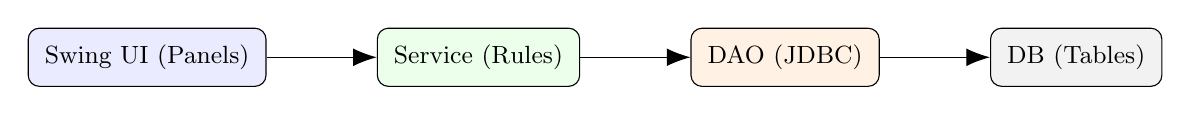
\begin{tikzpicture}[node distance=1.4cm, every node/.style={font=\small}]
    \node[draw, rounded corners, fill=blue!8, inner sep=6pt] (ui) {Swing UI (Panels)};
    \node[draw, rounded corners, fill=green!8, right=of ui, inner sep=6pt] (svc) {Service (Rules)};
    \node[draw, rounded corners, fill=orange!10, right=of svc, inner sep=6pt] (dao) {DAO (JDBC)};
    \node[draw, rounded corners, fill=gray!10, right=of dao, inner sep=6pt] (db) {DB (Tables)};
    \draw[-{Latex[length=3mm]}] (ui) -- (svc);
    \draw[-{Latex[length=3mm]}] (svc) -- (dao);
    \draw[-{Latex[length=3mm]}] (dao) -- (db);
  \end{tikzpicture}

  \vspace{0.6em}
  \begin{itemize}[<+->]
    \item UI: read inputs, show messages.
    \item Service: validation + business rules.
    \item DAO: SQL + mapping only.
  \end{itemize}
  \slidesources{\OOPSUnitVISources}
\end{frame}

\begin{frame}{Deliverable-3 (today)}
  \begin{itemize}[<+->]
    \item \texttt{schema.sql} committed to repo.
    \item At least 1--2 entities with DAO CRUD (minimum: insert + list).
    \item A small runner (\texttt{main}) that proves DAO works.
    \item Evidence: issues + PR + commit history.
  \end{itemize}
  \slidesources{\OOPSUnitVISources}
\end{frame}

\section{Key Topics}
\label{sec:concepts}

\begin{frame}{Unit 06: Capstone Project}
  \begin{itemize}[<+->]
    \item Lecture focus: Database Design + JDBC Layer
  \end{itemize}
  \slidesources{\OOPSUnitVISources}
\end{frame}

\begin{frame}{Today: Roadmap}
  \begin{itemize}[<+->]
    \item Entity model $\rightarrow$ relational schema (PK/FK, constraints)
    \item JDBC basics: connection, prepared statement, result set mapping
    \item DAO pattern + deliverable checklist
  \end{itemize}
  \slidesources{\OOPSUnitVISources}
\end{frame}

\begin{frame}{Entity model $\rightarrow$ tables (rule of thumb)}
  \begin{enumerate}[<+->]
    \item One entity class $\rightarrow$ one table.
    \item Fields $\rightarrow$ columns with types (\texttt{INT}, \texttt{VARCHAR}, \texttt{TIMESTAMP}).
    \item 1-to-many $\rightarrow$ FK column on the ``many'' side.
    \item Many-to-many $\rightarrow$ join table (two FKs).
  \end{enumerate}
  \slidesources{\OOPSUnitVISources}
\end{frame}

\begin{frame}{Keys + constraints (minimum)}
  \begin{itemize}[<+->]
    \item \textbf{PK}: unique row id (often auto-increment integer).
    \item \textbf{FK}: reference to another table's PK (maintains relationship).
    \item \textbf{NOT NULL}: required fields.
    \item \textbf{UNIQUE}: prevent duplicates (e.g., resource name).
  \end{itemize}
  \slidesources{\OOPSUnitVISources}
\end{frame}

\begin{frame}[fragile]{Example schema (Resource Booking) (1/2)}
\begin{lstlisting}[language=]
CREATE TABLE resources (
  id INT AUTO_INCREMENT PRIMARY KEY,
  name VARCHAR(100) NOT NULL UNIQUE,
  type VARCHAR(50) NOT NULL,
  capacity INT NOT NULL
);
\end{lstlisting}
  \slidesources{\OOPSUnitVISources}
\end{frame}

\begin{frame}[fragile]{Example schema (Resource Booking) (2/2)}
\begin{lstlisting}[language=]
-- continued...
CREATE TABLE bookings (
  id INT AUTO_INCREMENT PRIMARY KEY,
  resource_id INT NOT NULL,
  user_name VARCHAR(100) NOT NULL,
  start_time TIMESTAMP NOT NULL,
  end_time TIMESTAMP NOT NULL,
  status VARCHAR(20) NOT NULL,
  CONSTRAINT fk_booking_resource
    FOREIGN KEY (resource_id) REFERENCES resources(id)
);
\end{lstlisting}
  \slidesources{\OOPSUnitVISources}
\end{frame}

\begin{frame}{JDBC building blocks (3 objects)}
  \begin{itemize}[<+->]
    \item \texttt{Connection}: session with DB.
    \item \texttt{PreparedStatement}: parameterized SQL (safe + reusable).
    \item \texttt{ResultSet}: rows returned by a query.
  \end{itemize}
  \vspace{0.6em}
  \textbf{Rule:} close everything using \texttt{try-with-resources}.
  \slidesources{\OOPSUnitVISources}
\end{frame}

\begin{frame}[fragile]{PreparedStatement pattern (insert)}
\begin{lstlisting}
String sql = "INSERT INTO resources(name,type,capacity) VALUES(?,?,?)";
try (Connection con = DbUtil.getConnection();
     PreparedStatement ps = con.prepareStatement(sql)) {
    ps.setString(1, r.getName());
    ps.setString(2, r.getType());
    ps.setInt(3, r.getCapacity());
    ps.executeUpdate();
}
\end{lstlisting}
  \slidesources{\OOPSUnitVISources}
\end{frame}

\begin{frame}[fragile]{Mapping ResultSet $\rightarrow$ objects (select)}
\begin{lstlisting}
String sql = "SELECT id,name,type,capacity FROM resources";
List<Resource> out = new ArrayList<>();
try (Connection con = DbUtil.getConnection();
     PreparedStatement ps = con.prepareStatement(sql);
     ResultSet rs = ps.executeQuery()) {
    while (rs.next()) {
        out.add(new Resource(
            rs.getInt("id"),
            rs.getString("name"),
            rs.getString("type"),
            rs.getInt("capacity")
        ));
    }
}
\end{lstlisting}
  \slidesources{\OOPSUnitVISources}
\end{frame}

\begin{frame}{When do you need transactions?}
  \begin{itemize}[<+->]
    \item When one user action triggers \textbf{multiple} SQL statements.
    \item Example: create booking \textbf{and} update resource availability.
    \item If any step fails: rollback to keep DB consistent.
  \end{itemize}
  \vspace{0.6em}
  \textbf{Idea:} \texttt{con.setAutoCommit(false);} then \texttt{commit()/rollback()}.
  \slidesources{\OOPSUnitVISources}
\end{frame}

\begin{frame}{Common mistakes (avoid)}
  \begin{itemize}[<+->]
    \item Building SQL using string concatenation (SQL injection risk).
    \item Not closing \texttt{ResultSet}/\texttt{Statement}/\texttt{Connection}.
    \item Putting SQL inside Swing button code (mixing layers).
    \item Committing DB passwords in Git.
  \end{itemize}
  \slidesources{\OOPSUnitVISources}
\end{frame}

\section{Demo / Example}
\label{sec:demo}

\begin{frame}{Demo plan (10--15 mins)}
  \begin{enumerate}[<+->]
    \item Run \texttt{schema.sql} to create tables.
    \item Run a tiny \texttt{main} that calls: \texttt{insert} then \texttt{findAll}.
    \item Verify in DB using \texttt{SELECT * FROM resources;}.
  \end{enumerate}
  \slidesources{\OOPSUnitVISources}
\end{frame}

\begin{frame}{Mini Exercises (5 mins)}
  \begin{enumerate}[<+->]
    \item Add a UNIQUE constraint: which column in \texttt{resources} should be unique?
    \item Write SQL to list bookings for a resource id.
    \item In a DAO method, where does mapping happen: service or DAO?
  \end{enumerate}
  \slidesources{\OOPSUnitVISources}
\end{frame}


\section{Summary}
\label{sec:summary}

\begin{frame}{Key Takeaways}
  \begin{itemize}[<+->]
    \item Start from entities and design tables with keys + constraints.
    \item DAO layer uses JDBC with prepared statements + mapping.
    \item Deliverable-3 makes UI integration straightforward.
  \end{itemize}
  \slidesources{\OOPSUnitVISources}
\end{frame}

\begin{frame}{Checkpoint Questions}
  \begin{enumerate}[<+->]
    \item Why prefer \texttt{PreparedStatement} over string concatenation?
    \item What is the role of a foreign key?
    \item What should be inside a DAO method vs a service method?
  \end{enumerate}
  \slidesources{\OOPSUnitVISources}
\end{frame}

\begin{frame}{Next Lecture Preview}
  \textbf{Next:} Swing UI Panels + integration (Deliverable-4)
  \vspace{0.6em}
  \begin{itemize}[<+->]
    \item Build screens/panels and connect them to your service/DAO.
    \item Implement one end-to-end flow: UI $\rightarrow$ DB $\rightarrow$ UI refresh.
  \end{itemize}
  \slidesources{\OOPSUnitVISources}
\end{frame}

\end{document}
